\let\negmedspace\undefined
\let\negthickspace\undefined
\documentclass[journal]{IEEEtran}
\usepackage[a5paper, margin=10mm, onecolumn]{geometry}

\usepackage{tfrupee} 
\setlength{\headheight}{1cm} 
\setlength{\headsep}{0mm}       

\usepackage{gvv-book}
\usepackage{gvv}
\usepackage{cite}
\usepackage{amsmath,amssymb,amsfonts,amsthm}
\usepackage{algorithmic}
\usepackage{graphicx}
\usepackage{textcomp}
\usepackage{xcolor}
\usepackage{txfonts}
\usepackage{listings}
\usepackage{enumitem}
\usepackage{mathtools}
\usepackage{gensymb}
\usepackage{comment}
\usepackage[breaklinks=true]{hyperref}
\usepackage{tkz-euclide} 
\usepackage{listings}

\def\inputGnumericTable{}                                 
\usepackage[latin1]{inputenc}                                
\usepackage{color}                                            
\usepackage{array}                                            
\usepackage{longtable}                                       
\usepackage{calc}                                             
\usepackage{multirow}                                         
\usepackage{hhline}                                           
\usepackage{ifthen}                                           
\usepackage{lscape}
\begin{document}
	
	\bibliographystyle{IEEEtran}
	\vspace{3cm}
	
	\title{4.13.57}
	\author{EE25BTECH11052 - Shriyansh Kalpesh Chawda}
	
	{\let\newpage\relax\maketitle}
	
	\renewcommand{\thefigure}{\theenumi}
	\renewcommand{\thetable}{\theenumi}
	\setlength{\intextsep}{10pt} 
	
	\numberwithin{equation}{enumi}
	\numberwithin{figure}{enumi}
	\renewcommand{\thetable}{\theenumi}
	\textbf{Question}:\\
Find the equation of the line passing through the point $(2,3)$ and making intercept of length 2 units between the lines $y + 2x = 3$ and $y + 2x = 5$. 
\hfill(1991)
\begin{figure}[H]
	\centering
	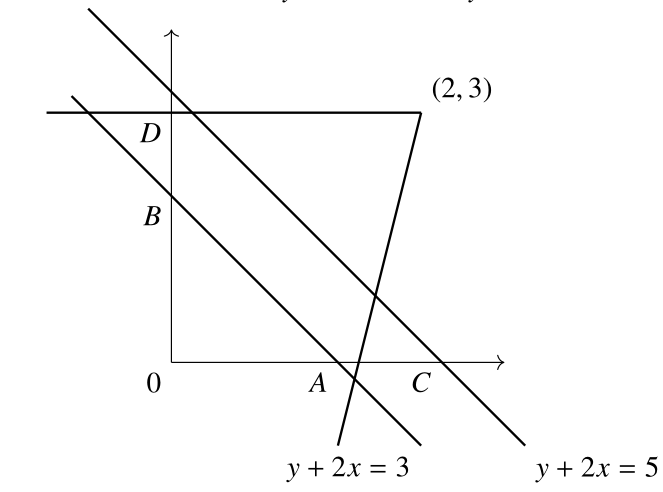
\includegraphics[width=0.4\linewidth]{figs/question}
	\caption{}
	\label{fig:question}
\end{figure}
\textbf{Solution}\\
The point is given by:
\[ \mathbf{P} = \myvec{2 \\ 3} \]
The two lines are expressed in the vector form $\vec{n} \cdot \vec{x} = d$.
\begin{align}
	\myvec{2 & 1} \myvec{x \\ y} = 3 \\
	\myvec{2 & 1} \myvec{x \\ y} = 5
\end{align}
The common normal vector is $\vec{n}$ and the distance constants $d_1$ and $d_2$:
\begin{align}
\vec{n} = \myvec{2 \\ 1}, \quad d_1 = 3, \quad d_2 = 5 \end{align}
The line passes through $\mathbf{P}$ with an unknown direction vector $\vec{v}$ is:
\begin{align} \vec{x} = \vec{P} + t\vec{v} = \myvec{2 \\ 3} + t \myvec{v_x \\ v_y} \end{align}
The unknown line intersect $L_1$ at point $\mathbf{B}$ (parameter $t_B$) and $L_2$ at point $\mathbf{D}$ (parameter $t_D$).
\begin{align}
	\mathbf{n} \cdot (\mathbf{P} + t_B \mathbf{v}) = d_1 &\implies t_B = \frac{d_1 - \mathbf{n} \cdot \mathbf{P}}{\mathbf{n} \cdot \mathbf{v}} \\
	\mathbf{n} \cdot (\mathbf{P} + t_D \mathbf{v}) = d_2 &\implies t_D = \frac{d_2 - \mathbf{n} \cdot \mathbf{P}}{\mathbf{n} \cdot \mathbf{v}}
\end{align}
Now ,Using the length of intercept.\\
\begin{align}
\|\vec{D} - \vec{B}\| = \|(\vec{P} + t_D \vec{v}) - (\vec{P} + t_B \vec{v})\| = |t_D - t_B| \cdot \|\vec{v}\| = 2
\end{align} 
Using (0.3) and (0.4)\\
\begin{align}
t_D - t_B = \frac{d_2 - \mathbf{n} \cdot \mathbf{P}}{\mathbf{n} \cdot \mathbf{v}} - \frac{d_1 - \mathbf{n} \cdot \mathbf{P}}{\mathbf{n} \cdot \mathbf{v}} = \frac{d_2 - d_1}{\mathbf{n} \cdot \mathbf{v}}
\end{align}
Substituting this into the distance equation:
\begin{align}
\left| \frac{d_2 - d_1}{\mathbf{n} \cdot \mathbf{v}} \right| \cdot \|\mathbf{v}\| = 2 \\
\frac{2}{|\mathbf{n} \cdot \mathbf{v}|} \cdot \|\mathbf{v}\| = 2 \implies \|\mathbf{v}\| = |\mathbf{n} \cdot \mathbf{v}| 
\end{align}
We express the condition $\|\mathbf{v}\| = |\mathbf{n} \cdot \mathbf{v}|$ as a matrix quadratic form. Squaring both sides gives:
\begin{align} 
&\|\mathbf{v}\|^2 = (\mathbf{n} \cdot \mathbf{v})^2 \\
&\mathbf{v}^\top\mathbf{I}\mathbf{v} = \mathbf{v}^\top(\mathbf{n}\mathbf{n}^\top)\mathbf{v} \\
&\mathbf{v}^\top\mathbf{I}\mathbf{v} - \mathbf{v}^\top(\mathbf{n}\mathbf{n}^\top)\mathbf{v} = 0\\
&\mathbf{v}^\top (\mathbf{n}\mathbf{n}^\top - \mathbf{I}) \mathbf{v} = 0, 
\end{align}
Let,
\begin{align}
\mathbf{Q} = \mathbf{n}\mathbf{n}^\top - \mathbf{I} = \myvec{2 \\ 1} \myvec{2 & 1} - \myvec{1 & 0 \\ 0 & 1} = \myvec{3 & 2 \\ 2 & 0} 
\end{align}
We now solve the quadratic form equation for $\mathbf{v} = \myvec{v_x \\ v_y}$:
\begin{align} \mathbf{v}^\top \mathbf{Q} \mathbf{v} = \myvec{v_x & v_y} \myvec{3 & 2 \\ 2 & 0} \myvec{v_x \\ v_y} = 0 \end{align}
\begin{align} 
3v_x^2 + 4v_xv_y = 0 \implies v_x(3v_x + 4v_y) = 0 
\end{align}
This yields two possible solutions for the components of the direction vector.\\
(a) $v_x = 0$ : \\The direction vector is vertical.Hence $\mathbf{v_1}$ and vertical line passing through the point $(2, 3)$ is :
\begin{align} 
	&\mathbf{v_1} = \myvec{0 \\ 1}\\
	&\mathbf{x} = 2 
\end{align}
(b) $3v_x + 4v_y = 0$ :\\ This implies \begin{align}
v_y = -\frac{3}{4}v_x\\
\mathbf{v_2} = \myvec{4 \\ -3}
\end{align}
So, corresponding to a slope of $m = -3/4$. Using the point-slope form :
\begin{align}
&y - 3 = -\frac{3}{4}(x - 2) \\
	&4(y - 3) = -3(x - 2) \\
	&4y - 12 = -3x + 6 \\
     &3x + 4y = 18
\end{align}
The two lines that satisfy the given conditions are :
\[	x = 2 \quad and\quad
3x + 4y = 18 \]

\begin{figure}[H]
	\centering
	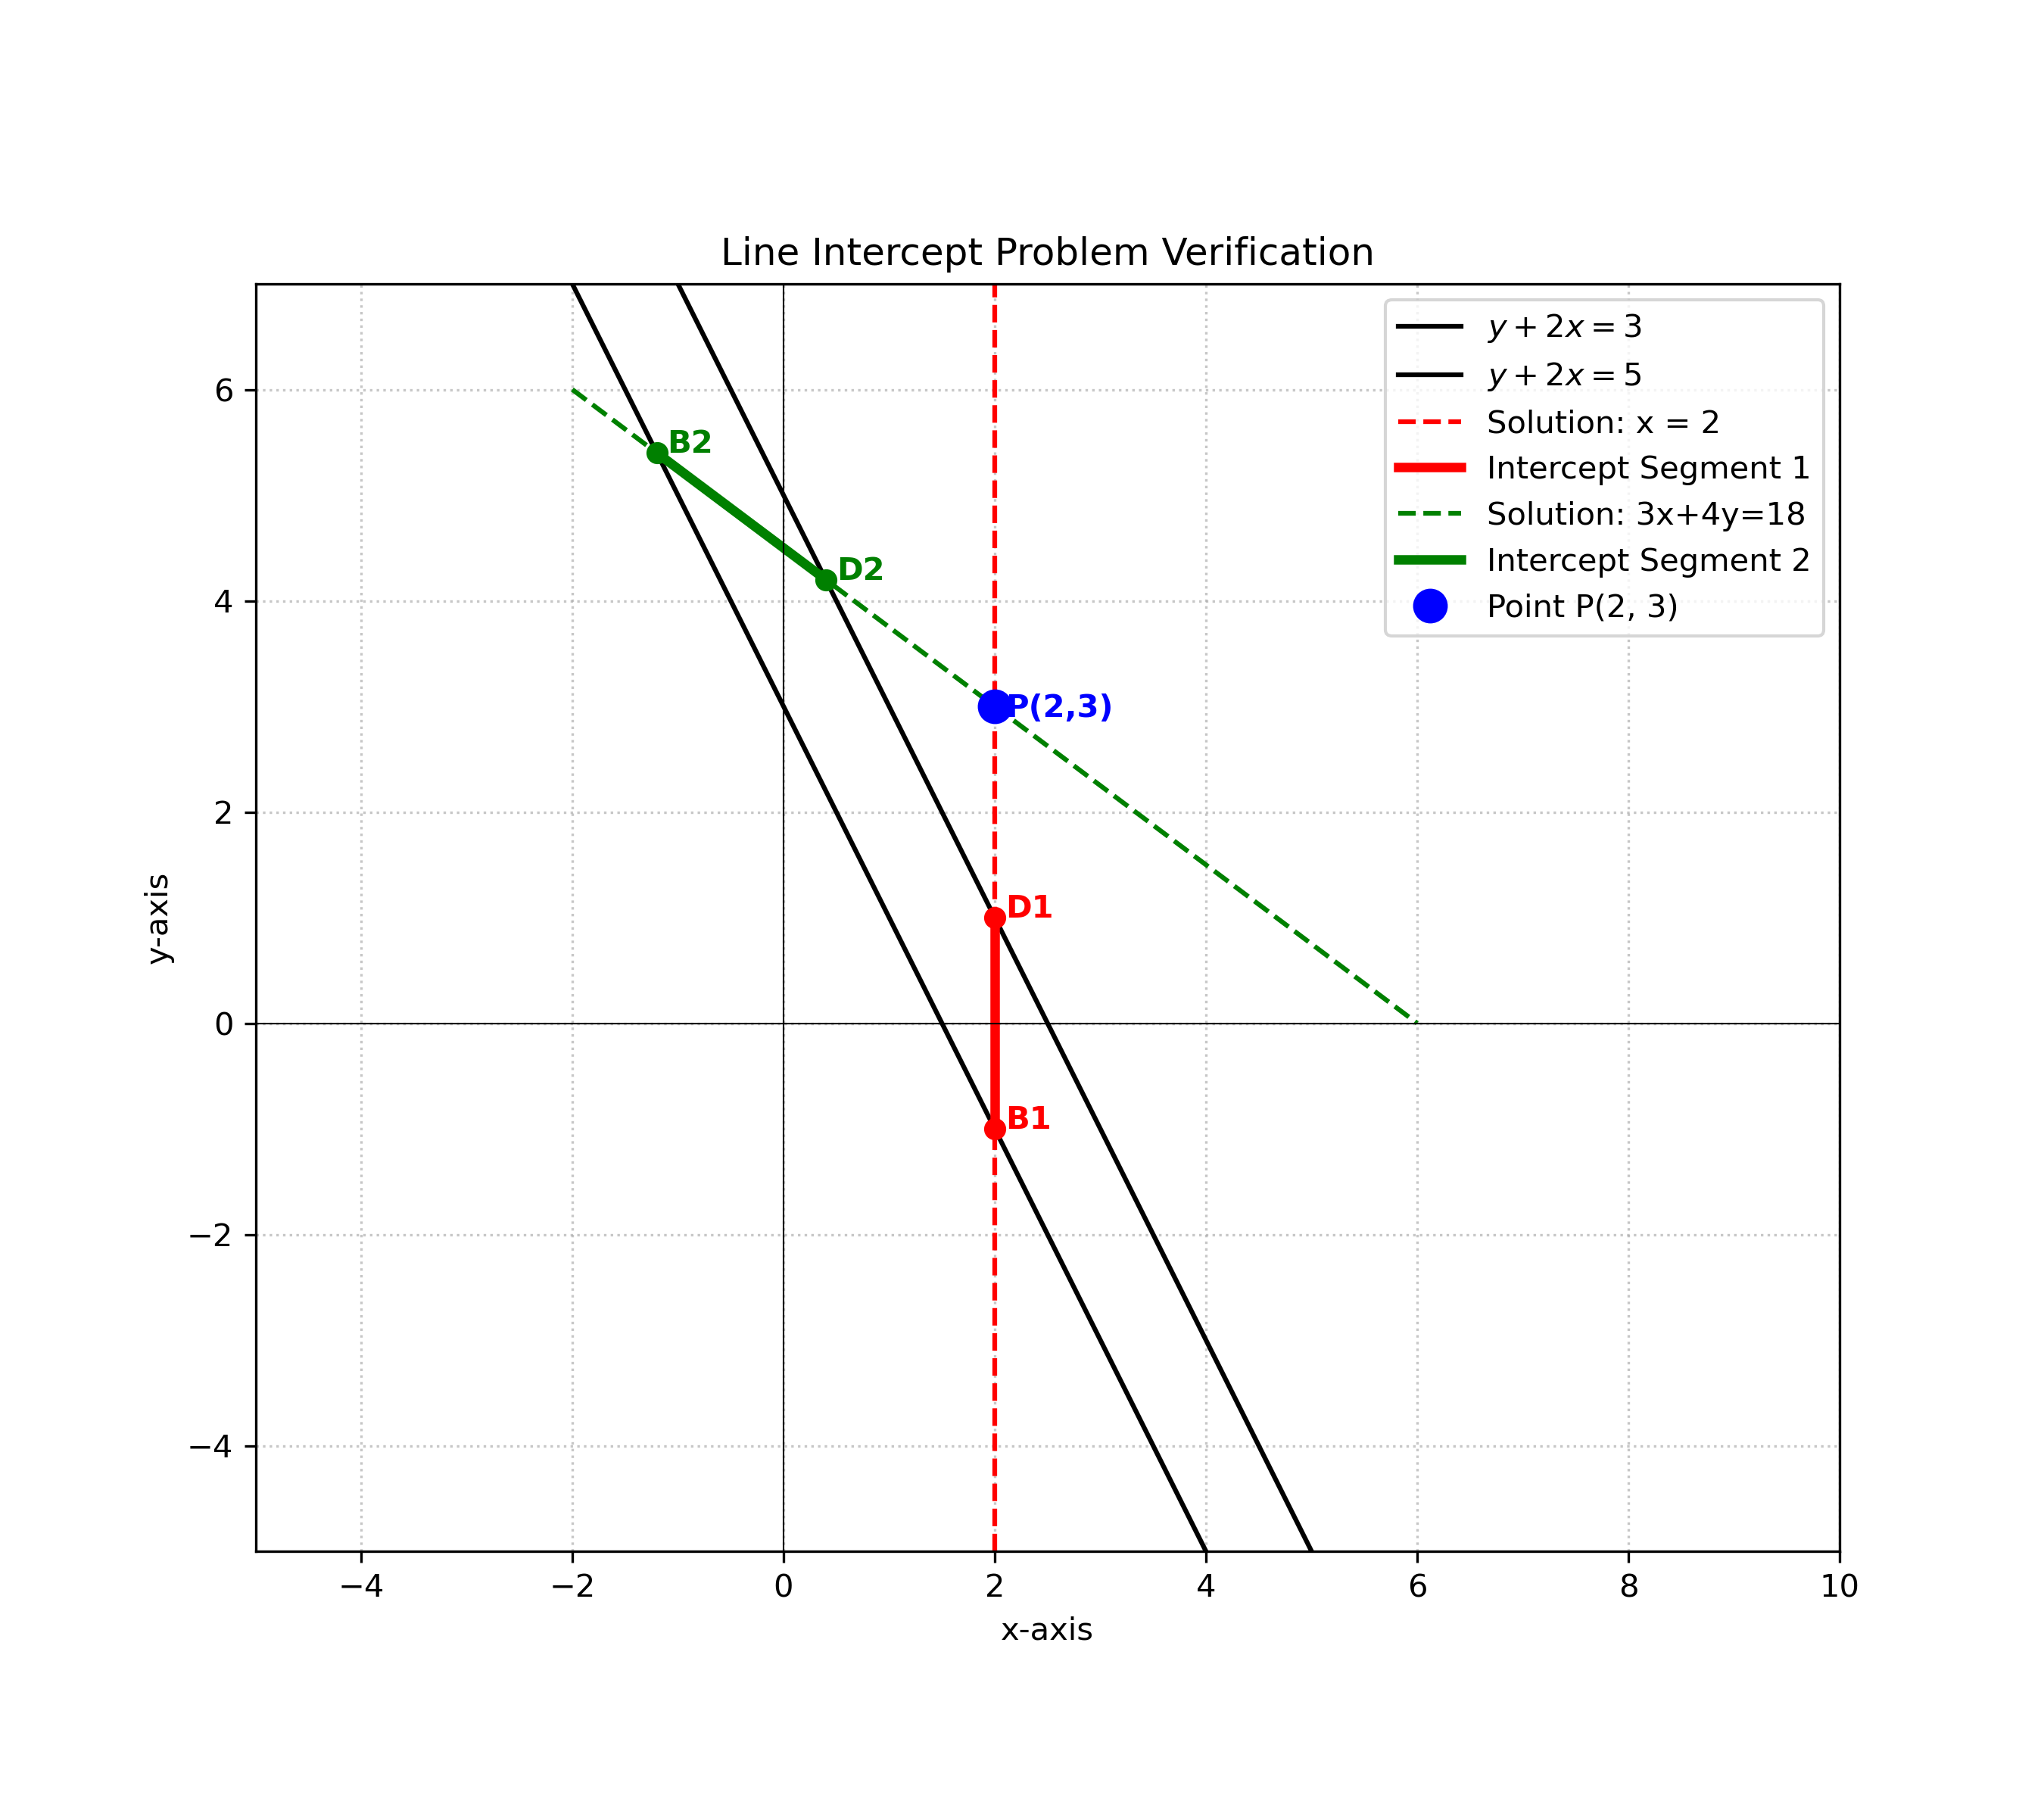
\includegraphics[width=1.1\linewidth]{figs/line_intercept_plot}
\end{figure}






\end{document}